\section{Prototype Implementation}
\label{sec:implementation}

We will now look into how the prototype is organized in the frontend and the backend.  This will hopefully show how our system works as a whole. We will focus more on the backend than the frontend in this section. 

\subsection{Frontend overview}
\noindent We will now look at our frontend and include main features, components, development tools and configuration. The frontend is responsible for displaying the backend as a UI (user interface). For our frontend we use SvelteKit with Vite and Tailwind.

\begin{figure}[H]
\centering
\resizebox{\textwidth}{!}{ % Resize the image to fit within the page width
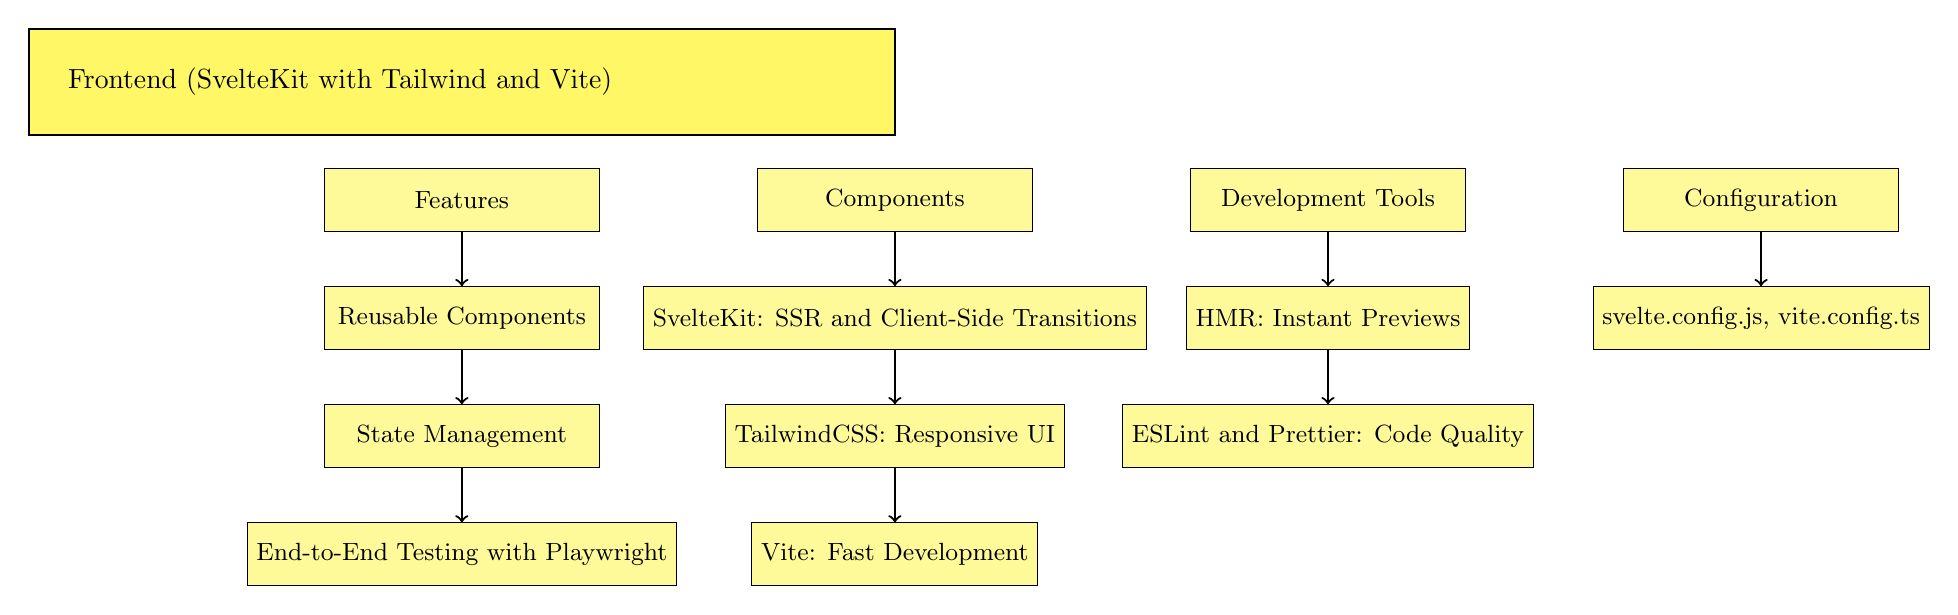
\begin{tikzpicture}[node distance=1.5cm, font=\small] % Set the font size for better visibility
\tikzstyle{container} = [draw=black, thick, inner sep=0.5cm] % Removed dashed line for container
\tikzstyle{label} = [font=\bfseries, text centered, minimum width=3.5cm]

% Define the top container for "Frontend Features and Components" with smaller font size and no dotted line
\node[container, fill=yellow!60, text width=10cm, minimum height=1cm, font=\normalsize] (Frontend) {
Frontend (SvelteKit with Tailwind and Vite)};

\vspace{1cm}

% Define node styles
\tikzstyle{class} = [rectangle, draw=black, fill=yellow!40, text centered, minimum height=0.8cm, minimum width=3.5cm]
\tikzstyle{arrow} = [->, thick, draw=black]
\tikzstyle{container} = [draw=black, thick, inner sep=0.5cm] % Removed dashed line for container
\tikzstyle{label} = [font=\bfseries, text centered, minimum width=3.5cm]

% Define categories under "Frontend Features and Components" with yellow boxes
\node[class, below of=Frontend, node distance=1.5cm] (Features) {Features};
\node[class, below of=Features] (ReusableComponents) {Reusable Components};
\node[class, below of=ReusableComponents] (StateManagement) {State Management};
\node[class, below of=StateManagement] (PlaywrightTesting) {End-to-End Testing with Playwright};

\node[class, right of=Features, xshift=4cm] (Components) {Components};
\node[class, below of=Components] (SvelteKit) {SvelteKit: SSR and Client-Side Transitions};
\node[class, below of=SvelteKit] (TailwindCSS) {TailwindCSS: Responsive UI};
\node[class, below of=TailwindCSS] (Vite) {Vite: Fast Development};

\node[class, right of=Components, xshift=4cm] (DevTools) {Development Tools};
\node[class, below of=DevTools] (HMR) {HMR: Instant Previews};
\node[class, below of=HMR] (CodeQuality) {ESLint and Prettier: Code Quality};

\node[class, right of=DevTools, xshift=4cm] (Config) {Configuration};
\node[class, below of=Config] (ConfigurationFiles) {svelte.config.js, vite.config.ts};

% Draw arrows between categories and elements
\draw[arrow] (Features) -- (ReusableComponents);
\draw[arrow] (ReusableComponents) -- (StateManagement);
\draw[arrow] (StateManagement) -- (PlaywrightTesting);

\draw[arrow] (Components) -- (SvelteKit);
\draw[arrow] (SvelteKit) -- (TailwindCSS);
\draw[arrow] (TailwindCSS) -- (Vite);

\draw[arrow] (DevTools) -- (HMR);
\draw[arrow] (HMR) -- (CodeQuality);

\draw[arrow] (Config) -- (ConfigurationFiles);

\end{tikzpicture}
}
\caption{Frontend Overview for PollApp Architecture (with Configuration)}
\label{fig:frontend_overview_with_configuration}
\end{figure}



\noindent \textbf{Framework:} SvelteKit for SSR and client-side transitions. \\
\noindent \textbf{Styling:} TailwindCSS for rapid, responsive UI design. \\
\noindent \textbf{Build Tools:} Vite for fast development and optimized builds. \\
\noindent \textbf{Key Features:} Organized structure for reusable components, state management, and static assets. End-to-end testing with Playwright ensures reliability. \\
\noindent \textbf{Development:} Hot Module Replacement (HMR) enables instant previews, while ESLint and Prettier maintain code quality. \\
\noindent  \textbf{Configuration:} Highly customizable via \texttt{svelte.config.js} and \texttt{vite.config.ts}.


\subsection{Backend overview}
We use Kotlin with Spring Boot as the backend. The code is organized into three main services: EventService, PollService, and UserService. These handle the business logic. We also have class JwtService,  which provides token management for authentication.
 
\begin{figure}[H]
\centering
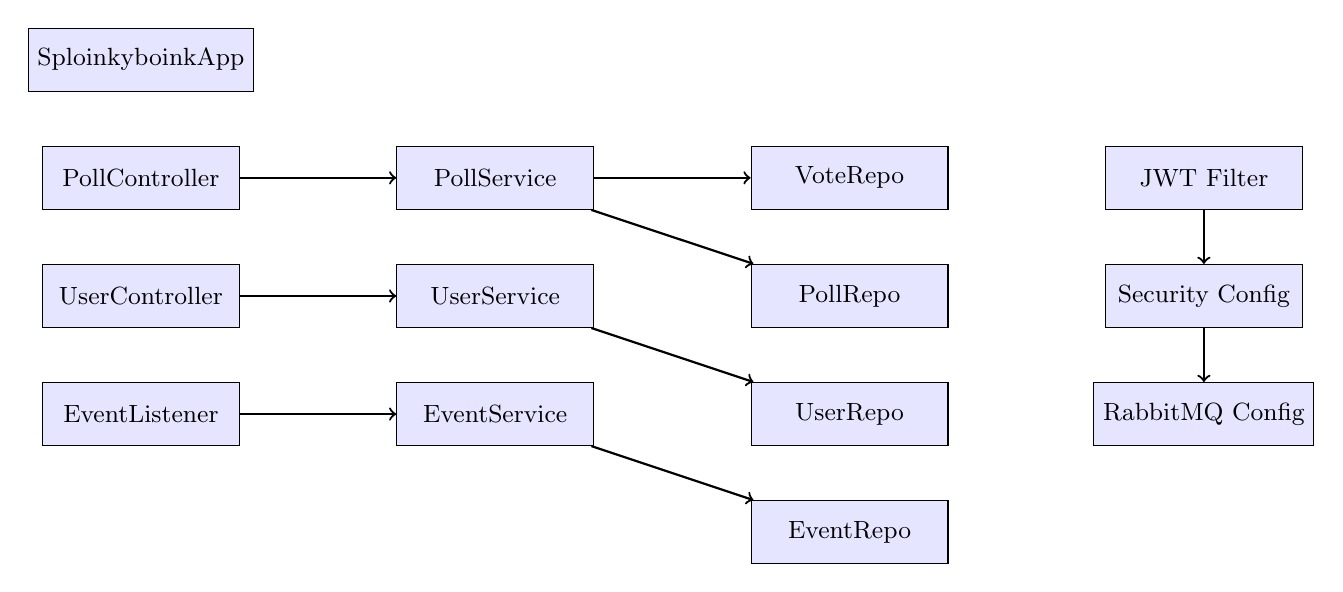
\begin{tikzpicture}[node distance=1.5cm, font=\small]
% Define UML class styles
\tikzstyle{class} = [rectangle, draw=black, fill=blue!10, text centered, minimum height=0.8cm, minimum width=2.5cm]
\tikzstyle{arrow} = [->, thick, draw=black]

% Define nodes (classes)
\node[class] (SploinkyboinkApplication) {SploinkyboinkApp};
\node[class, below of=SploinkyboinkApplication] (PollController) {PollController};
\node[class, below of=PollController] (UserController) {UserController};
\node[class, below of=UserController] (EventListener) {EventListener};

% Define second layer nodes (Services)
\node[class, right of=PollController, xshift=3cm] (PollService) {PollService};
\node[class, below of=PollService] (UserService) {UserService};
\node[class, below of=UserService] (EventService) {EventService};

% Define third layer nodes (Repositories)
\node[class, right of=PollService, xshift=3cm] (VoteRepository) {VoteRepo};
\node[class, below of=VoteRepository] (PollRepository) {PollRepo};
\node[class, below of=PollRepository] (UserRepository) {UserRepo};
\node[class, below of=UserRepository] (EventRepository) {EventRepo};

% Define fourth layer nodes (Security)
\node[class, right of=VoteRepository, xshift=3cm] (JwtAuthFilter) {JWT Filter};
\node[class, below of=JwtAuthFilter] (SecurityConfig) {Security Config};

% Define fifth layer nodes (Configurations)
\node[class, below of=SecurityConfig] (RabbitMQConfig) {RabbitMQ Config};

% Relationships (arrows)
\draw[arrow] (PollController) -- (PollService);
\draw[arrow] (UserController) -- (UserService);
\draw[arrow] (EventListener) -- (EventService);
\draw[arrow] (PollService) -- (PollRepository);
\draw[arrow] (PollService) -- (VoteRepository);
\draw[arrow] (UserService) -- (UserRepository);
\draw[arrow] (EventService) -- (EventRepository);
\draw[arrow] (JwtAuthFilter) -- (SecurityConfig);
\draw[arrow] (SecurityConfig) -- (RabbitMQConfig);

\end{tikzpicture}

\caption{Overview of the architecture in regards to controllers, services, repositories, and configurations}
\label{fig:controller_service_repo_config}
\end{figure}
\vspace{1cm}


\vspace{0.5cm}
\noindent \textbf{Achieved functionalities}
\begin{itemize}
    \item \textbf{Polling Functionality}: Users can create, manage, and participate in polls, with their votes accurately captured and stored.
    \item \textbf{Event Tracking}: Tracks important user actions, enabling auditing or analytics.
    \item \textbf{User Management}: Ensures secure user authentication and management through validation mechanisms.
    \item \textbf{Integration with Messaging}: RabbitMQ integration supports a scalable, event-driven architecture, enabling the decoupling of services and enhancing overall application performance.
\end{itemize}